% --- shared colours (matplotlib tab10) ---
\definecolor{cblue}{RGB}{31,119,180}
\definecolor{cred}{RGB}{214,39,40}
\definecolor{cgreen}{RGB}{44,160,44}

% common picture options: 1 bit = 0.042 cm on both axes (square aspect)
\tikzset{bitsec/.style={x=0.042cm,y=0.042cm,font=\small}}

%======================================================================
% PANEL 1 :  log t  vs  log eps   (advantage view)  --  SEARCH / linear
%======================================================================
\newcommand{\panelEpsSearch}{%
  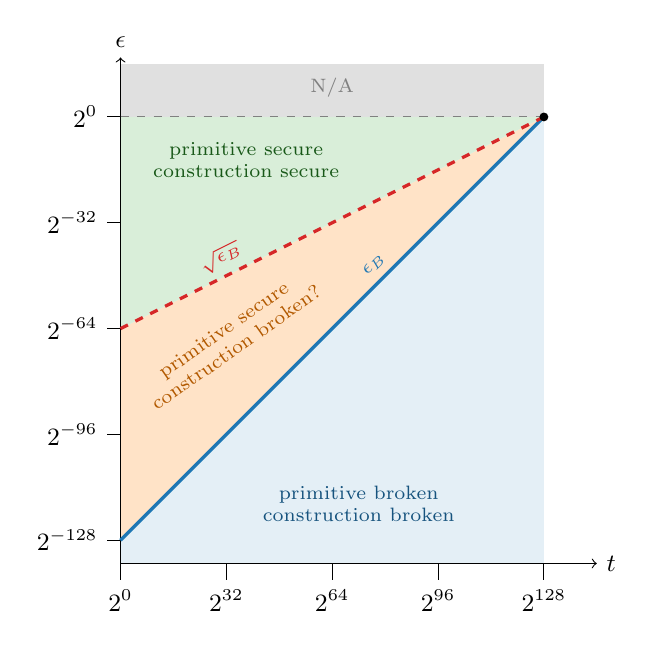
\begin{tikzpicture}[bitsec]
    \def\n{128}
    \fill[black!12]   (0,0) -- (0,16) -- (\n,16) -- (\n,0) -- cycle;
    \fill[cblue!12]  (0,-\n) -- (\n,0) -- (\n,-135) -- (0,-135) -- cycle;
    \fill[orange!22] (0,-\n) -- (0,{-\n/2}) -- (\n,0) -- cycle;
    \fill[cgreen!18] (0,{-\n/2}) -- (0,0) -- (\n,0) -- cycle;
    \draw[->] (0,-135) -- (0,18) node[above] {$\epsilon$};
    \draw[->] (0,-135) -- ({\n+16},-135) node[right] {$t$};
    \foreach \x in {0,32,64,96,128} \draw (\x,-135)--(\x,-140) node[below] {$2^{\x}$};
    \foreach \y in {0,-32,-64,-96,-128} \draw (0,\y)--(-4,\y) node[left] {$2^{\y}$};
    %\node[gray,rotate=90,anchor=south,font=\scriptsize] at (-24,-68) {$\downarrow$ more secure};
    \draw[gray,dashed] (0,0) -- (\n,0);
    \node[gray,font=\scriptsize] at ({0.5*\n},9) {N/A};
    \draw[cblue,very thick] (0,-\n) -- (\n,0);
    \draw[cred,very thick,dashed] (0,{-\n/2}) -- (\n,0);
    \fill (\n,0) circle (1.6pt);
    \node[cblue,rotate=45,anchor=south,font=\scriptsize] at (80,-48) {$\epsilon_B$};
    \node[cred,rotate=26.57,anchor=south,font=\scriptsize] at (33,-48) {$\sqrt{\epsilon_B}$};
    \node[cgreen!55!black,align=center,font=\scriptsize] at (38,-13) 
      {primitive secure \\ construction secure};
    \node[orange!70!black,rotate=35,align=center,font=\scriptsize] at (33,-67)
      {primitive secure \\ construction broken?};
    \node[cblue!70!black,align=center,font=\scriptsize] at (72,-117) 
      {primitive broken \\ construction broken};
  \end{tikzpicture}
}

%======================================================================
% PANEL 2 :  log t  vs  log eps   --  GROVER / collision
%======================================================================
\newcommand{\panelEpsGrover}{%
  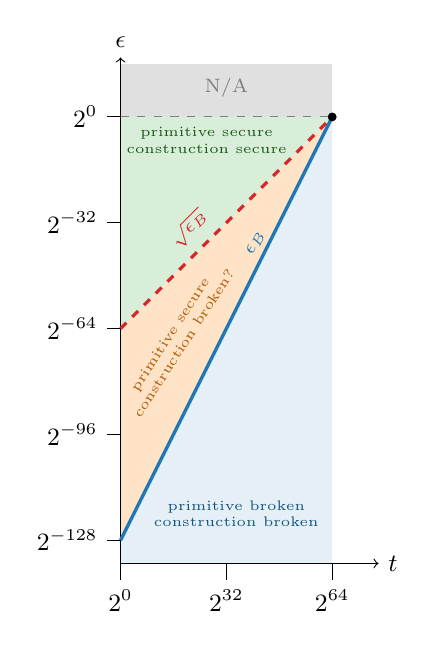
\begin{tikzpicture}[bitsec]
    \def\n{128}\def\m{64}
    \fill[black!12]   (0,0) -- (0,16) -- (\m,16) -- (\m,0) -- cycle;
    \fill[cblue!12]  (0,-\n) -- (\m,0) -- (\m,-135) -- (0,-135) -- cycle;
    \fill[orange!22] (0,-\n) -- (0,-\m) -- (\m,0) -- cycle;
    \fill[cgreen!18] (0,-\m) -- (0,0) -- (\m,0) -- cycle;
    \draw[->] (0,-135) -- (0,18) node[above] {$\epsilon$};
    \draw[->] (0,-135) -- ({\m+14},-135) node[right] {$t$};
    \foreach \x in {0,32,64} \draw (\x,-135)--(\x,-140) node[below] {$2^{\x}$};
    \foreach \y in {0,-32,-64,-96,-128} \draw (0,\y)--(-4,\y) node[left] {$2^{\y}$};
    \draw[gray,dashed] (0,0) -- (\m,0);
    \node[gray,font=\scriptsize] at (32,9) {N/A};
    \draw[cblue,very thick] (0,-\n) -- (\m,0);
    \draw[cred,very thick,dashed] (0,-\m) -- (\m,0);
    \fill (\m,0) circle (1.6pt);
    \node[cblue,rotate=63.43,anchor=south,font=\scriptsize] at (45,-40) {$\epsilon_B$};
    \node[cred,rotate=45,anchor=south,font=\scriptsize] at (25,-38) {$\sqrt{\epsilon_B}$};
    \node[cgreen!55!black,align=center,font=\tiny] at (26,-7) 
      {primitive secure \\ construction secure};
    \node[orange!70!black,rotate=57,align=center,font=\tiny] at (17,-67)
      {primitive secure \\ construction broken?};
    \node[cblue!70!black,align=center,font=\tiny] at (35,-120) 
      {primitive broken \\ construction broken};
  \end{tikzpicture}
}

%%% Invoking the Panels as Sub-Figures %%%
% Fixed scale + tabular  =>  Grover panel is literally half as wide,
% and the two x-axes align on a common baseline automatically.
\begin{tabular}{@{}c@{\hspace{3em}}c@{}}
  \panelEpsSearch & \panelEpsGrover\\[3pt]
  {\small (a) Best attack $=$ Brute-force search} & {\small (b) Best attack $=$ Grover search}\\
\end{tabular}
